% Disposição e ligações do gabinete — junta o croqui (croqui-tcc.drawio.png)
% e a aba "barramento" de "Imgs/Montagem croqui.xlsx". Fotos recortadas em
% Imgs/Metodologia/croqui/.
\begin{tikzpicture}[>=Stealth,
  every node/.append style={font=\fontsize{7}{8}\selectfont},
  borne/.style={draw, fill=#1, minimum width=0.72cm, minimum height=2.3cm, inner sep=1pt},
  borne/.default=white,
  bloco/.style={draw, thick, rounded corners=2pt, fill=white, align=center, minimum height=0.9cm, inner sep=3pt},
  foto/.style={inner sep=0pt},
  rot/.style={align=center, font=\fontsize{6.5}{7.5}\selectfont},
  fio/.style={thick, ->},
  pot/.style={line width=1.5pt, red!70!black},
  fase/.style={line width=1.2pt, orange!80!black},
  cmd/.style={thick, ->, dashed, blue!60!black},
  eth/.style={thick, green!50!black},
  sobre/.style={preaction={draw=black!3, line width=4pt, -}}]

  % ---------------- gabinete ----------------
  \draw[very thick, rounded corners=4pt, fill=black!3] (-0.9,-5.4) rectangle (14.6,8.4);
  \node[anchor=north west, font=\fontsize{8}{9}\selectfont\bfseries] at (-0.8,8.3) {Gabinete};

  % ---------------- régua de bornes ----------------
  \node[foto] (din) at (-0.05,0.3) {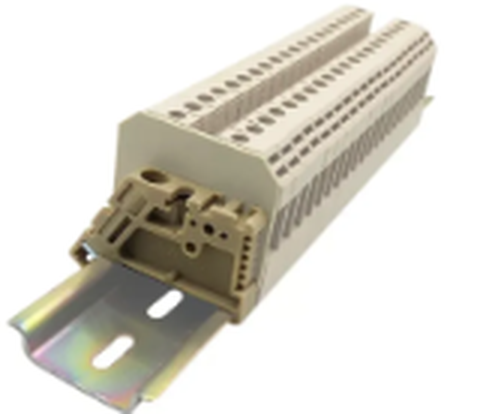
\includegraphics[width=1.2cm]{Textuais/Imgs/Metodologia/croqui/din.png}};
  \node[rot, below=0pt of din, font=\fontsize{5.5}{6.5}\selectfont] {régua\\de bornes};
  \foreach \i/\net/\cor in {1/GND/gray!30, 2/5 V/orange!25, 3/12 V/red!20,
                            4/5 V placas/orange!25, 5/GND placas/gray!30,
                            6/livre/white, 7/livre/white, 8/livre/white,
                            9/Pré-carga $+$/cyan!20, 10/Pré-carga $-$/gray!30,
                            11/Potência $+$/cyan!20, 12/Potência $-$/gray!30,
                            13/BAT$+$/red!35} {
    \pgfmathsetmacro{\x}{1.5+0.9*(\i-1)}
    \node[borne=\cor] (b\i) at (\x,0) {};
    \node[rotate=90] at ([yshift=-1.5mm]b\i.center) {\net};
    \node[font=\fontsize{6}{7}\selectfont\bfseries, below=1pt of b\i.north] {\i};
  }

  % ---------------- alimentação (acima, à esquerda) ----------------
  \node[foto] (fonte) at (1.9,4.0) {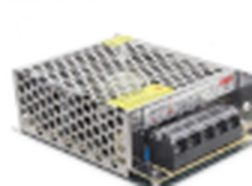
\includegraphics[width=1.9cm]{Textuais/Imgs/Metodologia/croqui/fonte.png}};
  \node[rot, below=1pt of fonte] {Fonte CA/CC 12 V};
  \node[foto] (buck) at (4.6,4.0) {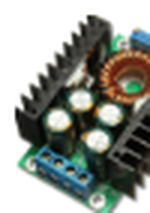
\includegraphics[width=1.1cm]{Textuais/Imgs/Metodologia/croqui/buck.png}};
  \node[rot, below=1pt of buck] {\textit{Buck} 12$\to$5 V};
  \draw[fio] (fonte.east) -- (buck.west);
  \draw[fio] ([xshift=-4mm]fonte.south) ++(0,-0.35) |- ++(0,-0.6) -| (b1.north);
  \draw[fio] ([xshift=4mm]fonte.south) ++(0,-0.35) -- ++(0,-1.0) -| (b3.north);
  \draw[fio] (buck.south) ++(0,-0.4) -- ++(0,-1.4) -| (b2.north);

  % ---------------- potência (acima, à direita) ----------------
  \node[bloco, fill=cyan!8, minimum width=1.4cm] (rpre) at (8.95,3.2) {Relé de\\pré-carga};
  \node[bloco, fill=cyan!8, minimum width=1.4cm] (rpot) at (10.75,3.2) {Relé de\\potência};
  \draw[thick] (b9.north)  -- ++(0,0.4) -| ([xshift=-3mm]rpre.south);
  \draw[thick] (b10.north) -- ++(0,0.7) -| ([xshift=3mm]rpre.south);
  \draw[thick] (b11.north) -- ++(0,0.4) -| ([xshift=-3mm]rpot.south);
  \draw[thick] (b12.north) -- ++(0,0.7) -| ([xshift=3mm]rpot.south);

  \node[foto] (esc) at (12.6,6.9) {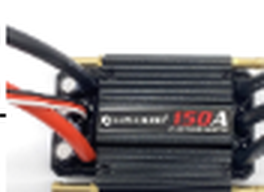
\includegraphics[width=1.9cm]{Textuais/Imgs/Metodologia/croqui/esc.png}};
  \node[rot, below=1pt of esc] {ESC};
  \node[bloco, minimum width=1.6cm] (aq1) at (8.0,6.9) {AQ1\\{\fontsize{6}{7}\selectfont tensões e correntes}};
  \node[foto] (motor) at (8.0,9.9) {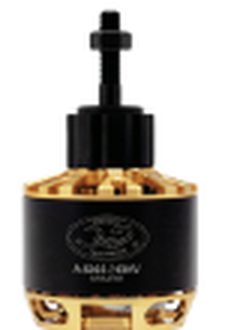
\includegraphics[height=1.6cm]{Textuais/Imgs/Metodologia/croqui/motor.png}};
  \node[rot, right=2pt of motor] {Motor BLDC};
  \foreach \d in {-2,0,2} {
    \draw[fase] ([yshift=\d mm]esc.west) -- ([yshift=\d mm]aq1.east);
    \draw[fase] ([xshift=\d mm]aq1.north) -- ([xshift=\d mm]motor.south);
  }
  \node[rot, above] at (10.3,7.15) {3 fases};

  % contatos: pré-carga passa pelo resistor; potência vai direto ao ESC
  \draw[pot] ([xshift=-4mm]rpre.north) to[R, l_={\SI{100}{\ohm}}] ++(0,2.0) |- ([yshift=-2mm]esc.south west);
  \draw[pot] ([xshift=4mm]rpot.north) |- ([yshift=-6mm]esc.south) -- ([yshift=-1mm]esc.south);
  \draw[pot, sobre] (b13.north) -- ++(0,2.85) -| ([xshift=-4mm]rpot.north);
  \draw[pot] ([xshift=-4mm]rpot.north) ++(0,0.42) -| ([xshift=4mm]rpre.north);
  \fill[red!70!black] ([xshift=-4mm]rpot.north) ++(0,0.42) circle (1.8pt);

  % ---------------- baixa tensão e rede (abaixo) ----------------
  \node[bloco, minimum width=1.4cm] (siba) at (3.6,-3.4) {SIBA};
  \node[bloco, minimum width=1.4cm] (sw)   at (5.5,-3.4) {\textit{Switch}\\de rede};
  \node[bloco, minimum width=1.4cm] (same) at (7.4,-3.4) {SAME};
  \draw[thick] (b4.south) -- ++(0,-0.35) -| (same.north);
  \draw[fio] (b4.south) ++(0,-0.35) -| (siba.north);
  \draw[fio] (sw.north |- 0,-1.5) -- (sw.north);
  \draw[fio] (same.north |- 0,-1.5) -- (same.north);
  \node[rot, anchor=north] at (6.5,-1.55) {5 V / GND};
  \draw[eth] (siba.east) -- (sw.west);
  \draw[eth] (same.west) -- (sw.east);
  \draw[dashed, gray] (aq1.west) -- ++(-2.9,0) node[rot, anchor=east, gray!70!black] {cabo de sinais para a SAME};

  \node[bloco, fill=red!10] (eme) at (1.6,-3.4) {Botão de\\emergência};
  \node[bloco] (mod) at (9.95,-3.4) {Módulos\\de relé (5 V)};
  \draw[fio] (b3.south) -- ++(0,-0.9) -| (eme.north);
  \draw[fio] (eme.south) -- ++(0,-1.2) -| ([xshift=4mm]mod.south);
  \node[rot, above] at (2.9,-5.05) {12 V após o botão};
  \draw[fio] ([xshift=-4mm]mod.north) |- ++(0,0.9) -| (b9.south);
  \draw[fio] ([xshift=4mm]mod.north) |- ++(0,0.9) -| (b11.south);
  \draw[cmd] (siba.south) -- ++(0,-0.75) -| ([xshift=-4mm]mod.south);
  \node[rot, above, blue!60!black] at (6.6,-4.6) {comando PB12 / PB13};

  \node[bloco, fill=red!10] (bat) at (12.3,-3.4) {Conector\\da bateria};
  \draw[pot] (bat.north) -- (b13.south);

  % ---------------- legenda ----------------
  \begin{scope}[shift={(0.3,-6.0)}]
    \draw[pot] (0,0) -- (0.6,0) node[right, rot] {potência (bateria)};
    \draw[fase] (3.0,0) -- (3.6,0) node[right, rot] {fases do motor};
    \draw[thick] (5.8,0) -- (6.4,0) node[right, rot] {alimentação 12/5 V};
    \draw[cmd] (8.8,0) -- (9.4,0) node[right, rot] {comando};
    \draw[eth] (11.0,0) -- (11.6,0) node[right, rot] {Ethernet};
  \end{scope}
\end{tikzpicture}
